% ==============================================================================
% PG - Lorenzo Rizzi Fiorot
% Capítulo 3 - O EduGraph
% ==============================================================================
% TODO(autor): o modelo do curso sugere que o título deste capítulo nomeie a
% contribuição do trabalho; "O EduGraph" é provisório.
\chapter{O EduGraph}
\label{sec-edugraph}

Texto.


%%% Início de seção. %%%
\section{Visão Geral}
\label{sec-edugraph-visao}

% TODO(autor): se houver requisitos registrados, eles entram nesta seção; senão, ela apresenta
% as funcionalidades tiradas do código.
Texto.

\begin{figure}[H]
    \centering
    \caption{Mapa de navegação entre as telas do EduGraph}
    \label{fig-mapa-telas}
    \marcadorbrasao
    \notafigura{aqui vai um mapa das telas, tipo um fluxograma: a home e as setas pra grafos, fórum, ontologias, arquiteturas pedagógicas, entrar e criar conta, mostrando que o header e o rodapé levam pra todas. dá pra fazer com caixinhas no latex.}
\end{figure}

\begin{table}[H]
    \centering
    \caption{Telas do EduGraph e o que o usuário faz em cada uma}
    \label{tab:funcionalidades}
    \renewcommand{\arraystretch}{1.3}
    \begin{tabular}{|l|l|}
        \hline
        \textbf{Tela} & \textbf{O que o usuário faz} \\
        \hline
        Texto. & Texto. \\
        \hline
    \end{tabular}
    \notafigura{aqui vai uma tabela com cada tela e o que dá pra fazer nela, tipo um resumo de tudo antes de entrar nos detalhes.}
\end{table}


%%% Início de seção. %%%
\section{Prototipação}
\label{sec-edugraph-prototipacao}

Texto.

\begin{figure}[H]
    \centering
    \caption{Protótipo inicial}
    \label{fig-prototipo-inicial}
    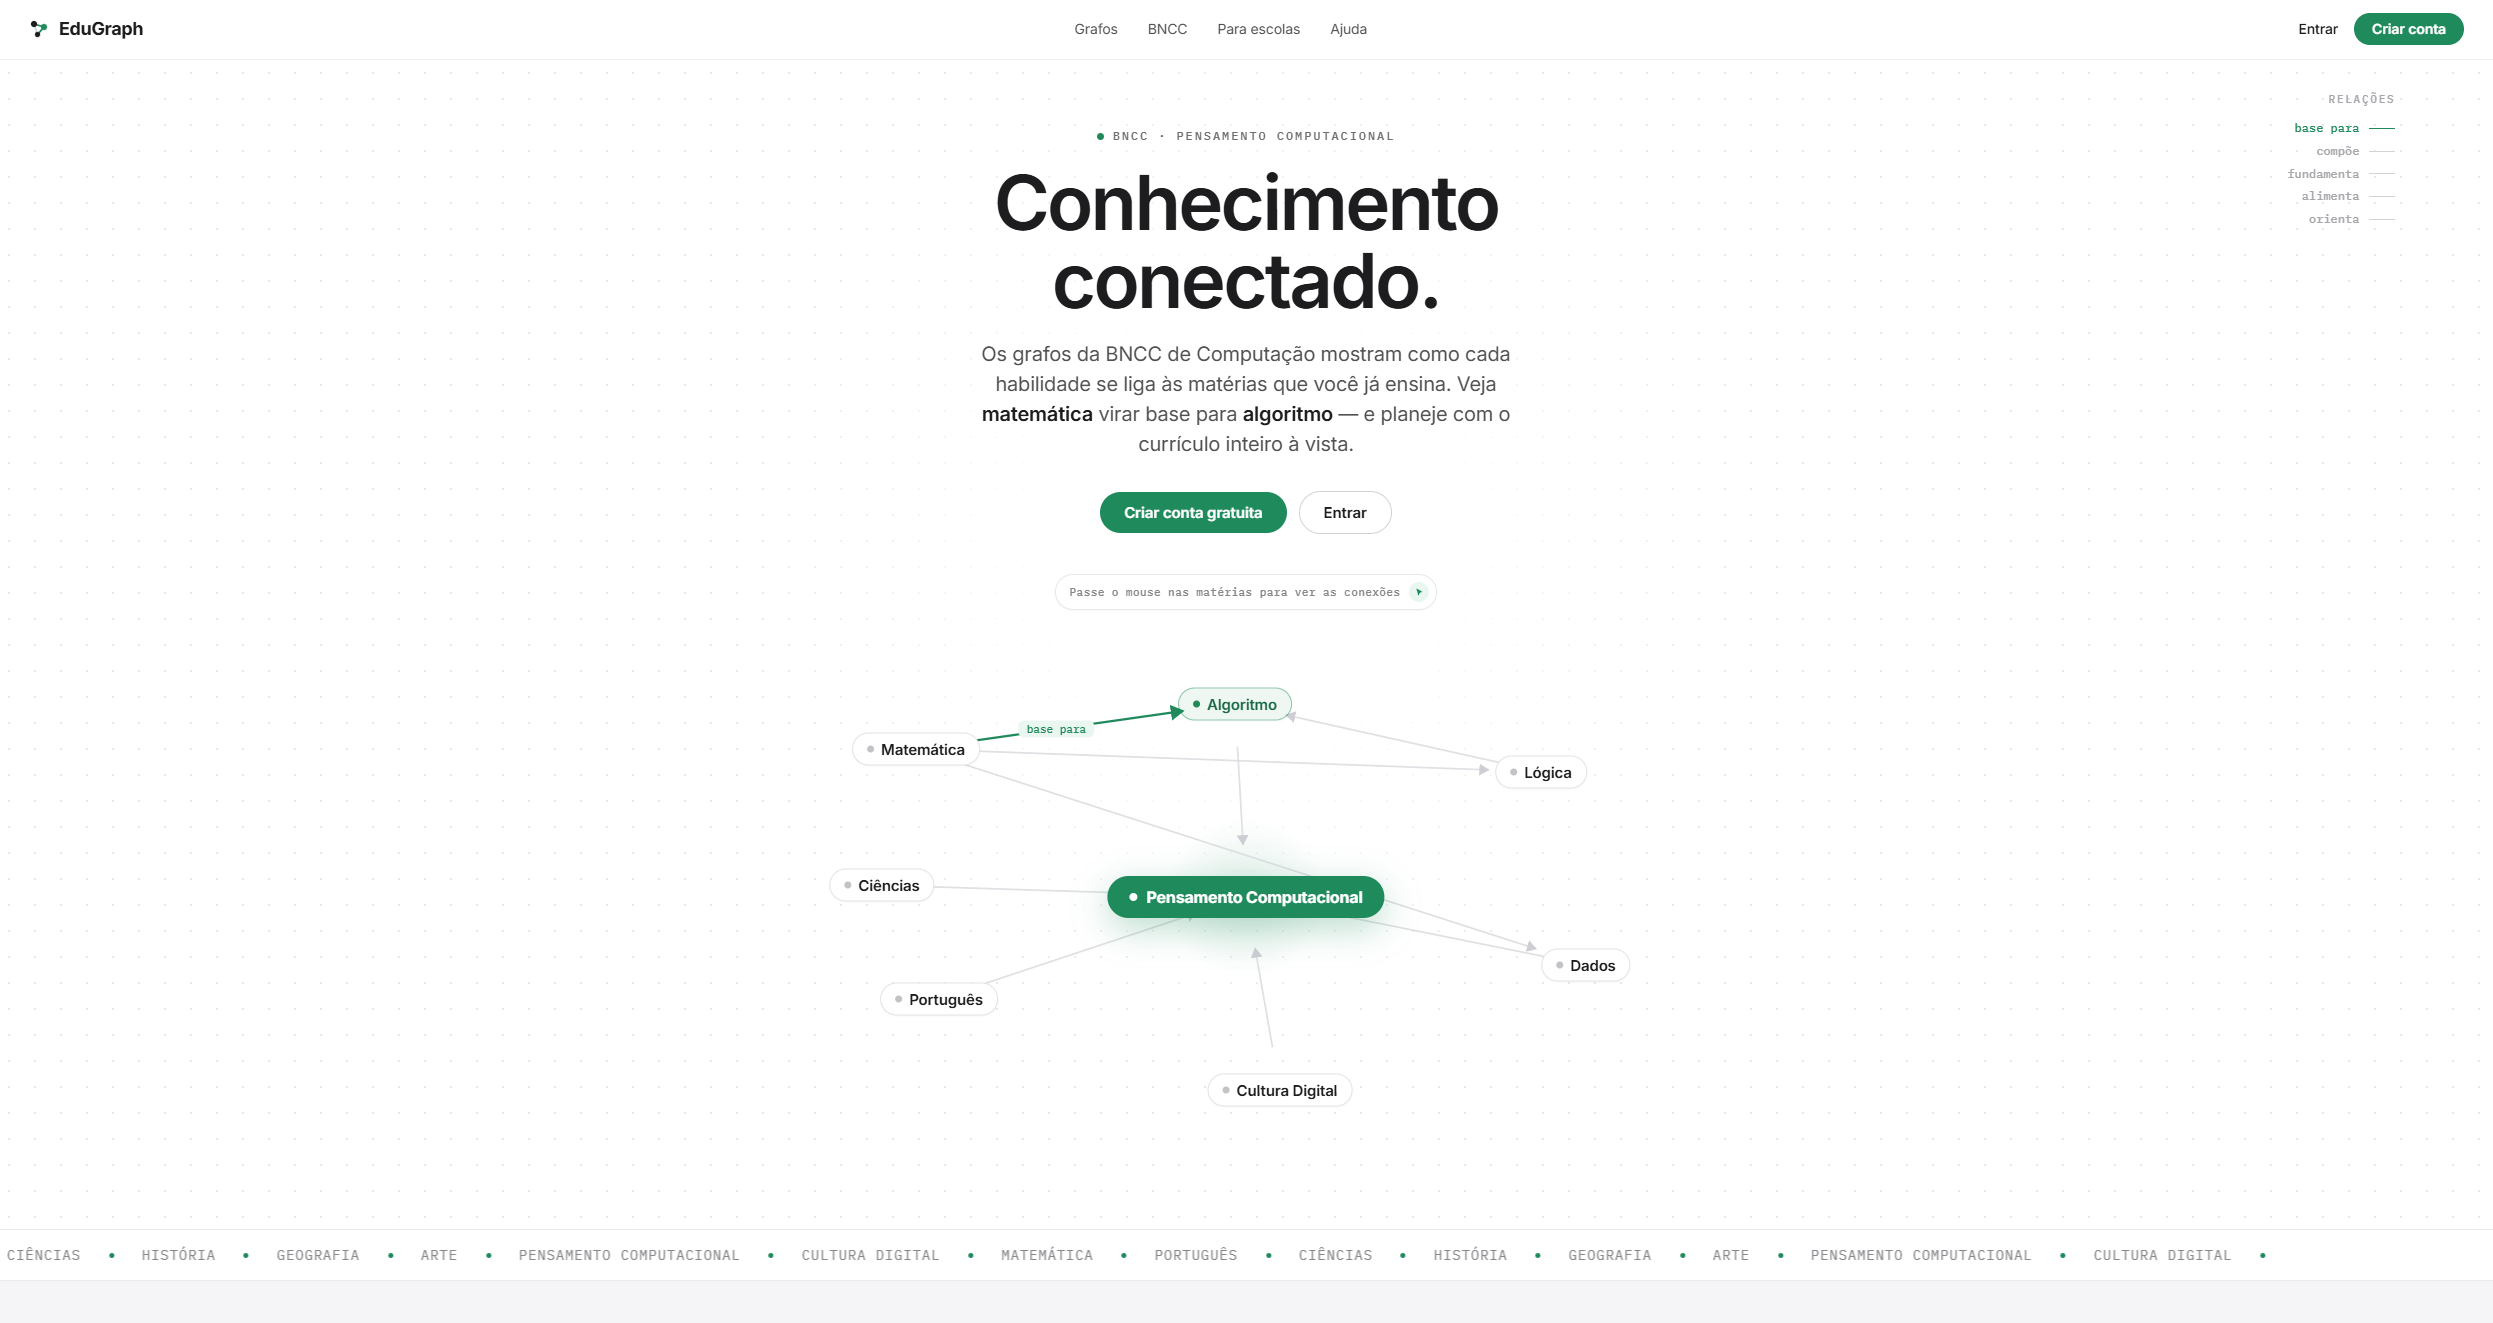
\includegraphics[width=\textwidth]{figuras/fig-prototipo-inicial.png}
\end{figure}

\begin{figure}[H]
    \centering
    \caption{Protótipo intermediário}
    \label{fig-prototipo-intermediario}
    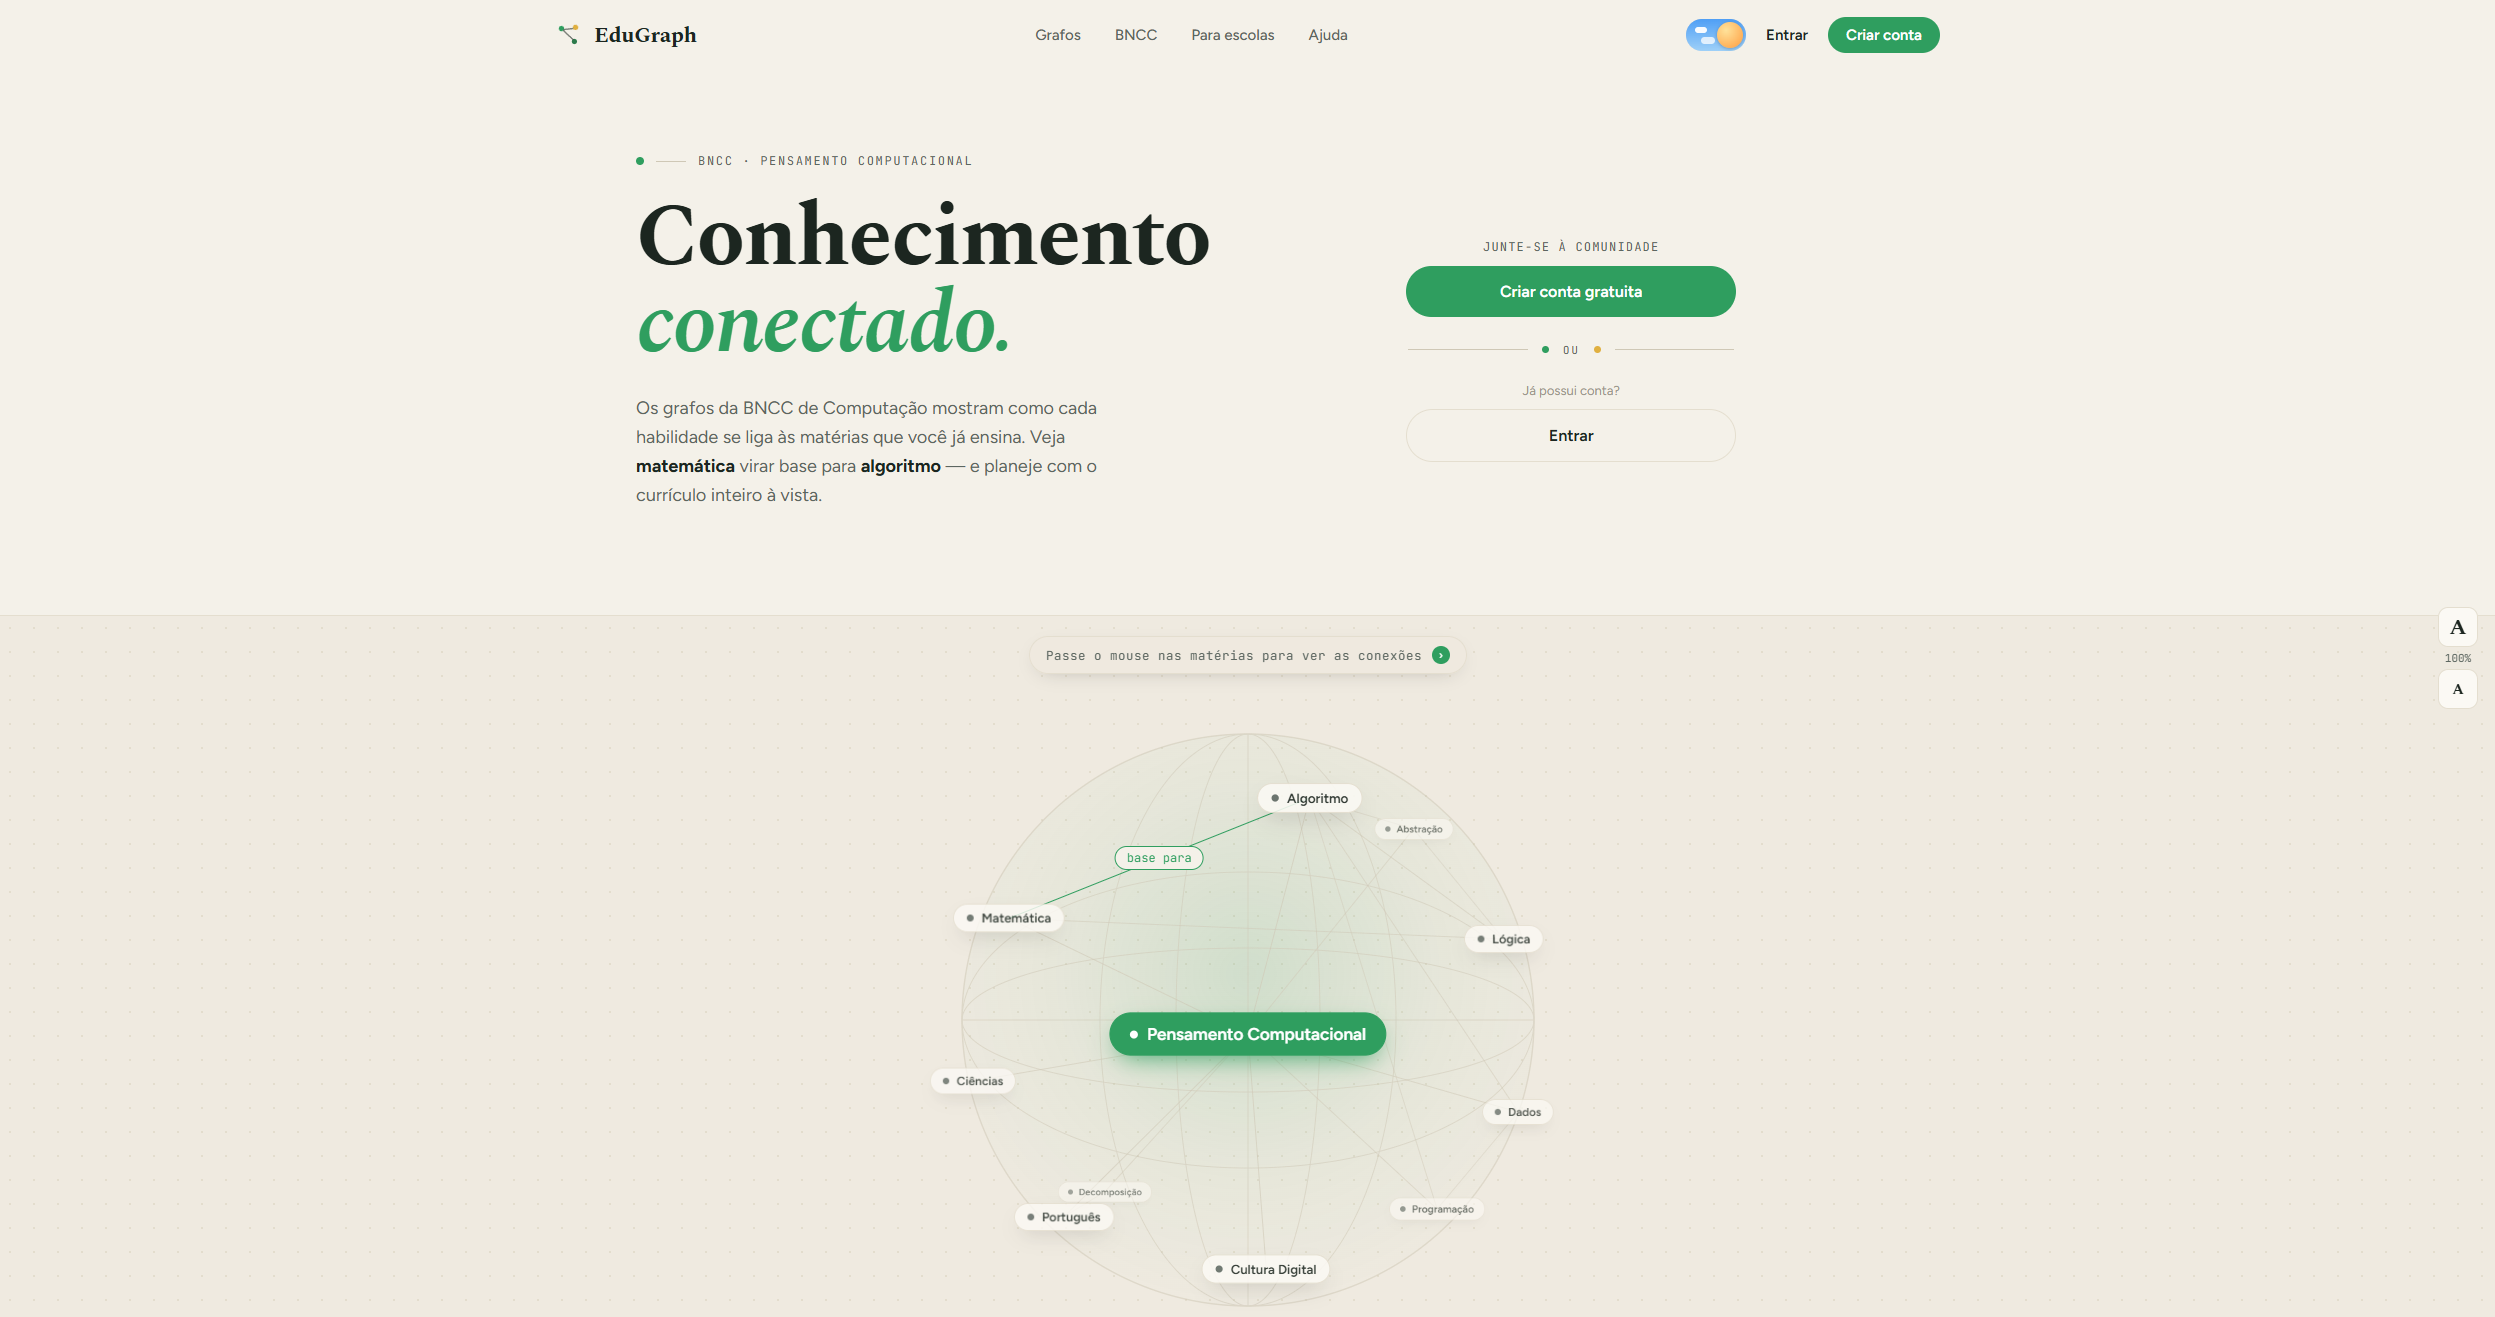
\includegraphics[width=\textwidth]{figuras/fig-prototipo-intermediario.png}
\end{figure}

\begin{figure}[H]
    \centering
    \caption{Protótipo final}
    \label{fig-prototipo-final}
    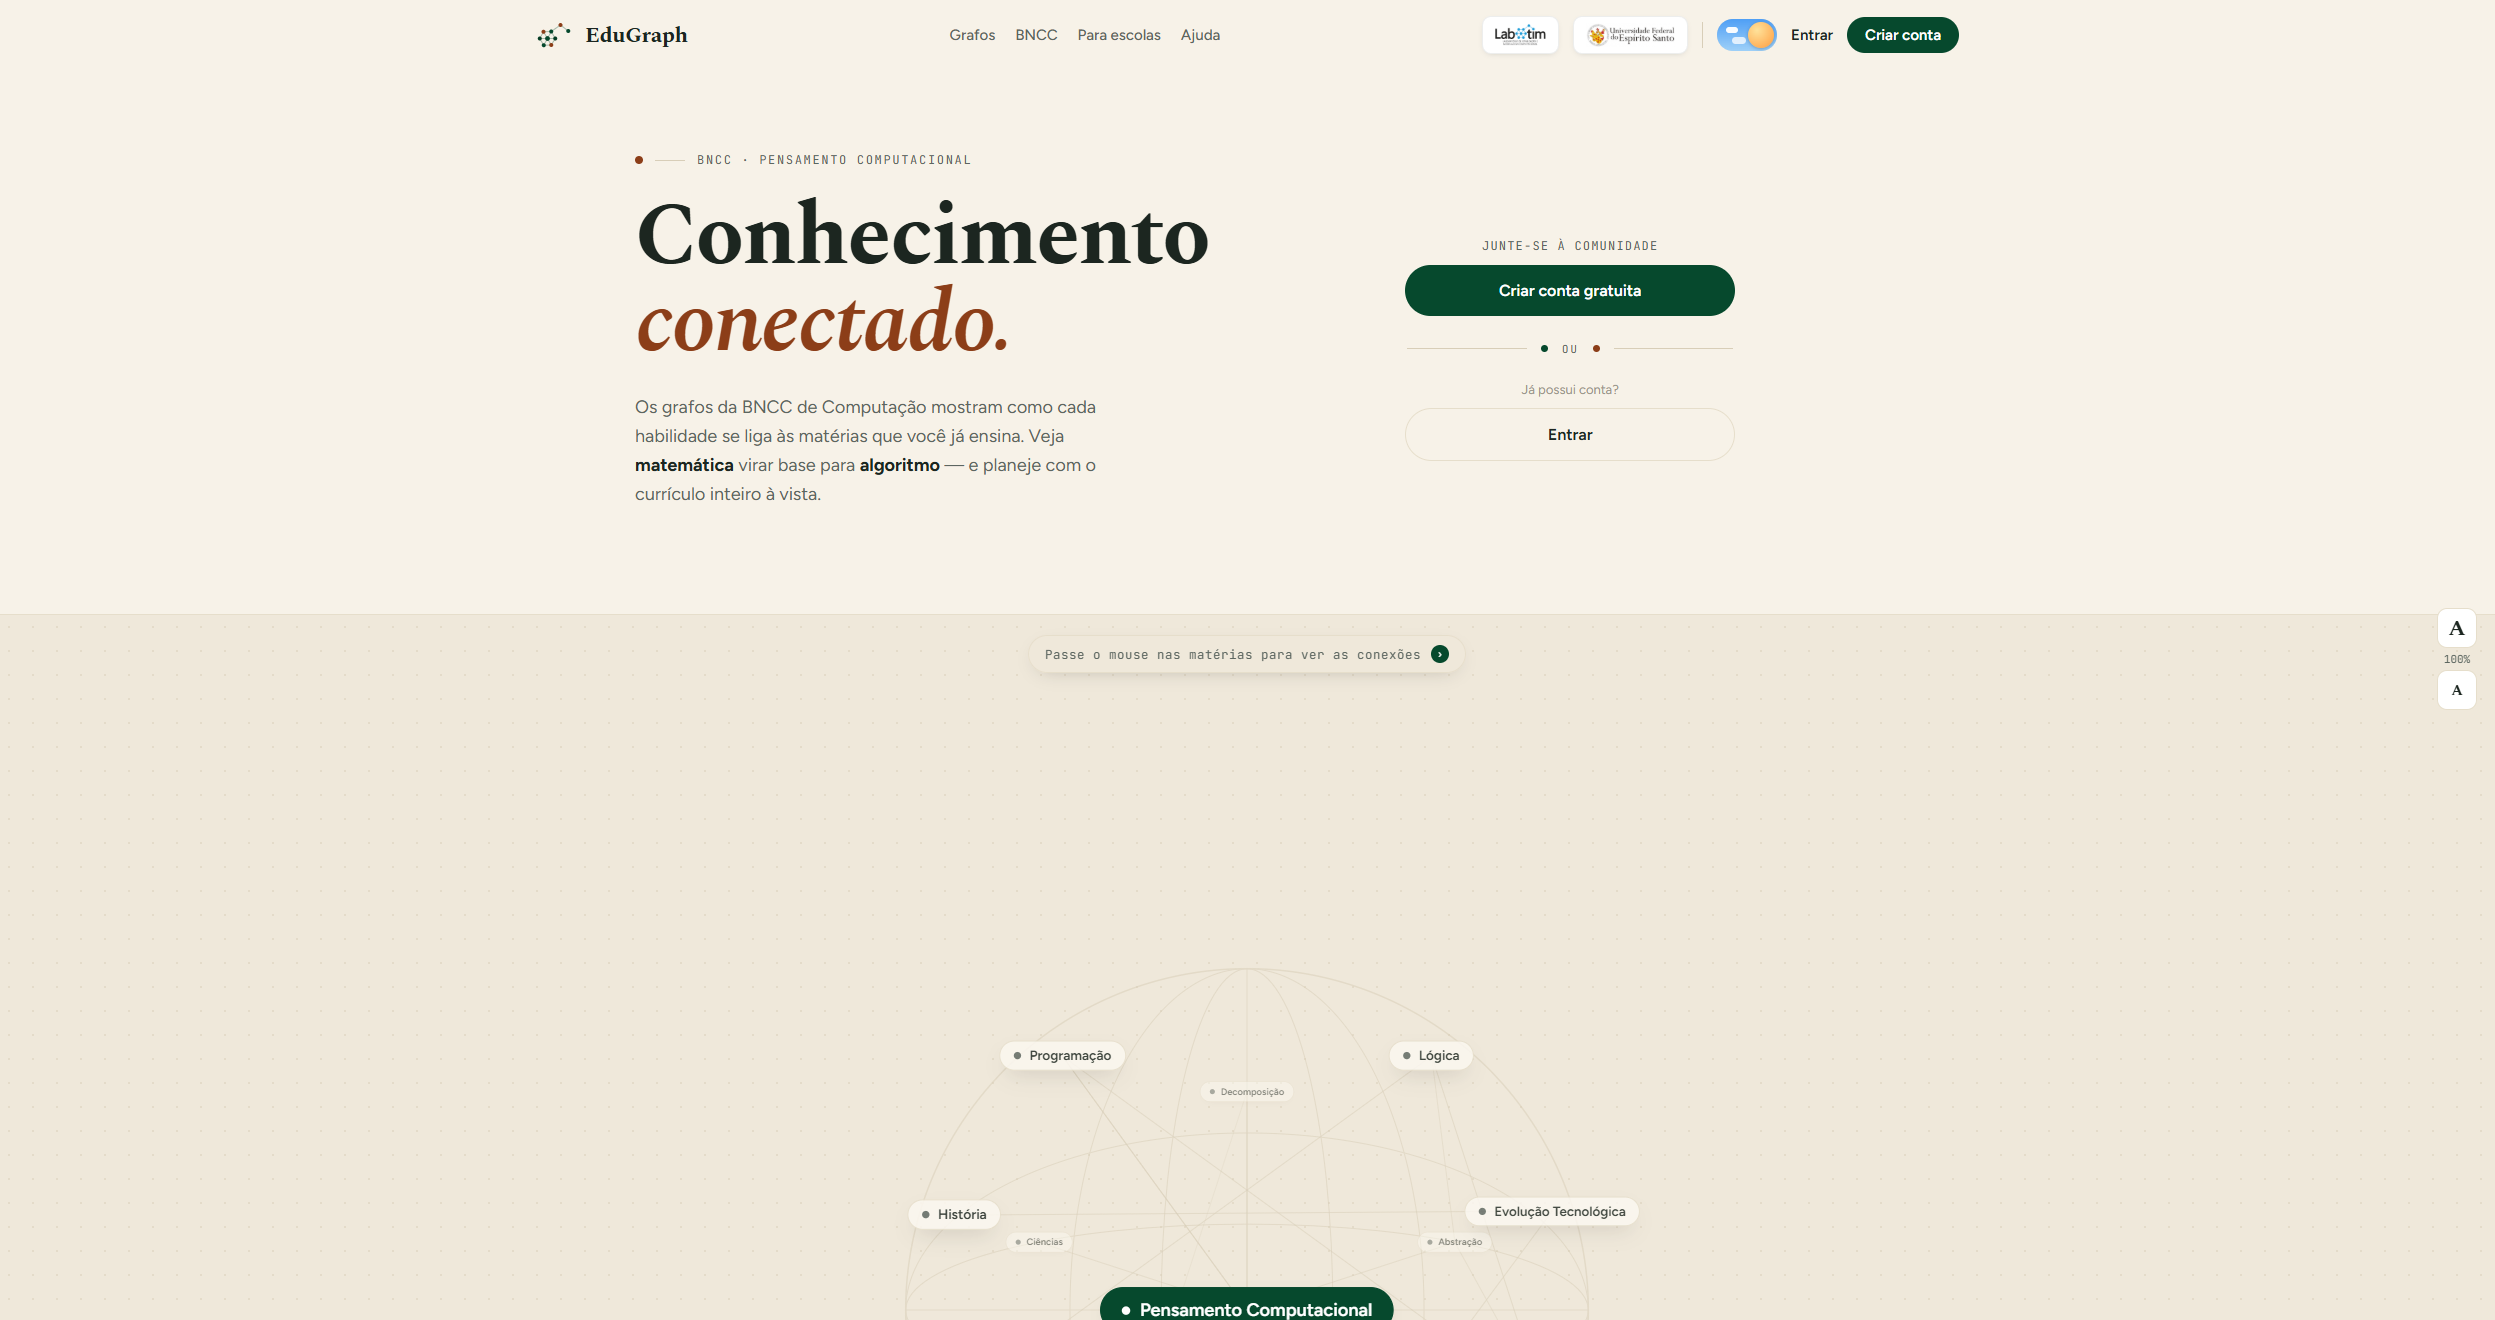
\includegraphics[width=\textwidth]{figuras/fig-prototipo-final.png}
\end{figure}


%%% Início de seção. %%%
\section{Arquitetura do Front-end}
\label{sec-edugraph-arquitetura}

Texto.

\begin{figure}[H]
    \centering
    \caption{Organização da aplicação web do EduGraph}
    \label{fig-arquitetura-front}
    \marcadorbrasao
    \notafigura{aqui vai um diagrama da organização do site: o app.jsx trocando as telas, as páginas, os componentes de cada página, os arquivos de dados e o tema (claro/escuro e tamanho da letra) valendo pra todo o site. a api e o banco aparecem só numa caixa pequena embaixo, porque não são o foco.}
\end{figure}

\begin{figure}[H]
    \centering
    \caption{Componentes da página de grafos}
    \label{fig-arvore-grafos}
    \marcadorbrasao
    \notafigura{aqui vai a árvore de componentes da página de grafos: a página em cima e embaixo a busca do professor, o canvas, o painel, a legenda, os controles e os estados (carregando e erro). pode ser uma árvore simples de caixinhas.}
\end{figure}

\begin{lstlisting}[caption={Trecho de um componente React do EduGraph},label={lst-componente}]
// trecho a definir
\end{lstlisting}
\notafigura{aqui vai um pedaço curto de código de verdade de um componente, tipo o item da navegação do header, pra mostrar como é um componente em react. curtinho, umas 15 linhas.}


%%% Início de seção. %%%
\section{Identidade Visual}
\label{sec-edugraph-identidade}

Texto.

\begin{table}[H]
    \centering
    \caption{Paleta de cores do EduGraph nos temas claro e escuro}
    \label{tab:paleta}
    \renewcommand{\arraystretch}{1.3}
    \begin{tabular}{|l|l|l|}
        \hline
        \textbf{Uso} & \textbf{Tema claro} & \textbf{Tema escuro} \\
        \hline
        Texto. & Texto. & Texto. \\
        \hline
    \end{tabular}
    \notafigura{aqui vai uma tabela com as cores do site: fundo, texto, verde, dourado e as outras, cada uma com um quadradinho da cor no tema claro e no escuro. as cores saem do index.css.}
\end{table}

\begin{figure}[H]
    \centering
    \caption{As três fontes do EduGraph em uso}
    \label{fig-tipografia}
    \captura[0.7\textwidth]{figuras/fig-tipografia.jpg}
    \notafigura{print já feito: o começo da home recortado, com as três fontes: a jetbrains mono no rótulo de cima, a spectral no título e a figtree no texto.}
\end{figure}

\begin{figure}[H]
    \centering
    \caption{A mesma tela nos temas claro e escuro}
    \label{fig-claro-escuro}
    \captura{figuras/fig-claro-escuro.jpg}
    \notafigura{print já feito: a home no tema claro, na esquerda, e no escuro, na direita, com a janela de 1600 por 1000.}
\end{figure}


%%% Início de seção. %%%
\section{Navegação e Elementos Comuns}
\label{sec-edugraph-navegacao}

Texto.

\begin{figure}[H]
    \centering
    \caption{Cabeçalho do site, com a navegação}
    \label{fig-header}
    \captura{figuras/fig-header.jpg}
    \notafigura{print já feito: o header saiu em duas linhas pra dar pra ler na página. em cima, o logo e a navegação; embaixo, os logos do labotim e da ufes, o botão de tema e o entrar/criar conta.}
\end{figure}

\begin{figure}[H]
    \centering
    \caption{Botão de troca de tema nos estados claro e escuro}
    \label{fig-tema-botao}
    \captura[0.45\textwidth]{figuras/fig-tema-botao.jpg}
    \notafigura{print já feito: o botão de tema bem de perto, com o sol no claro e a lua no escuro.}
\end{figure}

\begin{figure}[H]
    \centering
    \caption{Controle do tamanho da letra}
    \label{fig-fonte-widget}
    \captura[0.12\textwidth]{figuras/fig-fonte-widget.jpg}
    \notafigura{print já feito: o botãozinho do A/A na lateral, em 100\%.}
\end{figure}

\begin{figure}[H]
    \centering
    \caption{Rodapé do site}
    \label{fig-rodape}
    \captura{figuras/fig-rodape.jpg}
    \notafigura{print já feito: o rodapé inteiro, com as colunas plataforma e apoio e os logos embaixo.}
\end{figure}


%%% Início de seção. %%%
\section{Página Inicial}
\label{sec-edugraph-inicial}

Texto.

\begin{figure}[H]
    \centering
    \caption{Início da página inicial}
    \label{fig-home-hero}
    \captura{figuras/fig-home-hero.jpg}
    \notafigura{print já feito: a home logo no começo, tema claro, janela de 1600 por 1000.}
\end{figure}

\begin{figure}[H]
    \centering
    \caption{Seção ``Cada matéria tem sua rede'', com o globo de nós}
    \label{fig-home-globo}
    \captura{figuras/fig-home-globo.jpg}
    \notafigura{print já feito, em duas partes: na esquerda, o globo no começo da rolagem, com o mouse em cima de matemática e as conexões dela acesas; na direita, o globo depois de rolar, já de lado, com o texto da seção aparecendo.}
\end{figure}

\begin{figure}[H]
    \centering
    \caption{Faixa de números da página inicial}
    \label{fig-home-numeros}
    \captura{figuras/fig-home-numeros.jpg}
    \notafigura{print já feito: a faixa dos números já contados (36 habilidades, 8 unidades temáticas e o 1º e o 2º ano). esses números vêm do banco.}
\end{figure}

\begin{figure}[H]
    \centering
    \caption{Seção de depoimentos de professores}
    \label{fig-home-depoimentos}
    \captura{figuras/fig-home-depoimentos.jpg}
    \notafigura{print já feito: o desfile de depoimentos parado no segundo cartão.}
\end{figure}

\begin{figure}[H]
    \centering
    \caption{Grade das turmas, com o balão de componentes aberto}
    \label{fig-home-turmas}
    \captura{figuras/fig-home-turmas.jpg}
    \notafigura{print já feito: a grade das turmas com o balão do 1º ano aberto, mostrando ciências e matemática e o botão que leva pra busca já filtrada.}
\end{figure}


%%% Início de seção. %%%
\section{Página de Grafos}
\label{sec-edugraph-grafos}

Texto.


\subsection{Busca Guiada}
\label{sec-edugraph-grafos-busca}

Texto.

\begin{figure}[H]
    \centering
    \caption{Página de grafos antes da primeira busca}
    \label{fig-grafos-convite}
    \captura{figuras/fig-grafos-convite.jpg}
    \notafigura{print já feito: a página de grafos quando abre, com a busca em cima, o painel de contexto na esquerda e o cartão de boas-vindas no meio.}
\end{figure}

\begin{figure}[H]
    \centering
    \caption{Busca guiada, com a lista de um campo aberta}
    \label{fig-grafos-busca}
    \captura{figuras/fig-grafos-busca.jpg}
    \notafigura{print já feito: a busca com 1º ano, ciências da natureza, ciências e ``caminho até uma habilidade'', com a lista do campo filtrando pela palavra tempo.}
\end{figure}

\begin{figure}[H]
    \centering
    \caption{Estados de carregamento e de erro da página de grafos}
    \label{fig-grafos-estados}
    \captura{figuras/fig-grafos-estados.jpg}
    \notafigura{print já feito, em duas partes, só o palco: na esquerda, carregando; na direita, o cartão de erro de quando o servidor demora demais pra responder (tempo esgotado), com o tentar novamente.}
\end{figure}


\subsection{O Motor de Visualização em Canvas 2D}
\label{sec-edugraph-grafos-canvas}

Texto.

\begin{figure}[H]
    \centering
    \caption{Grafo desenhado no canvas pelo layout por forças}
    \label{fig-grafos-forcas}
    \captura{figuras/fig-grafos-forcas.jpg}
    \notafigura{print já feito: o ano inteiro de ciências do 1º ano no layout de forças, com o painel escondido.}
\end{figure}


\subsection{Layout por Forças e Layout Hierárquico}
\label{sec-edugraph-grafos-layouts}

Texto.

\begin{figure}[H]
    \centering
    \caption{O mesmo grafo no layout hierárquico}
    \label{fig-grafos-hierarquico}
    \captura{figuras/fig-grafos-hierarquico.jpg}
    \notafigura{print já feito: o mesmo grafo no layout hierárquico, com o ano em cima e as habilidades embaixo.}
\end{figure}


\subsection{Interações, Painel e Legenda}
\label{sec-edugraph-grafos-interacoes}

Texto.

\begin{figure}[H]
    \centering
    \caption{Painel de detalhe de uma habilidade}
    \label{fig-grafos-painel}
    \captura{figuras/fig-grafos-painel.jpg}
    \notafigura{print já feito: o EF01CI05 clicado, com o painel mostrando o texto da habilidade, as propriedades e as conexões. embaixo aparecem os vistos por último.}
\end{figure}

\begin{figure}[H]
    \centering
    \caption{Um nó antes e depois de expandido}
    \label{fig-grafos-expandir}
    \captura{figuras/fig-grafos-expandir.jpg}
    \notafigura{print já feito, em duas partes, só o palco: terra e universo selecionado, antes e depois dos dois cliques. depois chega um objeto do 2º ano e aparece o desfazer expansão.}
\end{figure}

\begin{figure}[H]
    \centering
    \caption{Legenda dos tipos de nó, com um tipo oculto}
    \label{fig-grafos-legenda}
    \captura{figuras/fig-grafos-legenda.jpg}
    \notafigura{print já feito: a legenda com objeto de conhecimento desligado e o desenho sem esses nós (12 nós, 3 ocultos).}
\end{figure}

\begin{figure}[H]
    \centering
    \caption{Menu do perfil, com as preferências de acessibilidade}
    \label{fig-grafos-perfil}
    \captura{figuras/fig-grafos-perfil.jpg}
    \notafigura{print já feito: o menu do perfil aberto, com as paletas pra daltonismo, as formas e o desligar animações.}
\end{figure}


\subsection{Do JSON ao Desenho}
\label{sec-edugraph-grafos-json}

Texto.

\begin{lstlisting}[caption={Trecho da resposta em JSON tipado recebida pelo site},label={lst-json}]
{ "$type": "Relationship",
  "_value": {
    "_element_id": "5:62285f86-914c-413d-8497-21f65e3bc508:87",
    "_start_node_element_id": "4:62285f86-914c-413d-8497-21f65e3bc508:52",
    "_end_node_element_id": "4:62285f86-914c-413d-8497-21f65e3bc508:57",
    "_type": "DESENVOLVE",
    "_properties": {} } },
{ "$type": "Node",
  "_value": {
    "_element_id": "4:62285f86-914c-413d-8497-21f65e3bc508:57",
    "_labels": ["HabilidadeCien"],
    "_properties": {
      "codigo": { "$type": "String", "_value": "EF01CI05" },
      "descricao": { "$type": "String",
        "_value": "Identificar e nomear diferentes escalas de tempo: os períodos diários (manhã, tarde, noite) e a sucessão de dias, semanas, meses e anos." } } } }
\end{lstlisting}
\notafigura{trecho de verdade da resposta da api pra busca ``caminho até uma habilidade'' com o EF01CI05: a última relação do caminho (DESENVOLVE) e o nó da habilidade, com o tipo de cada valor. só tirei a parte de antes do caminho.}

\begin{figure}[H]
    \centering
    \caption{Do JSON recebido ao grafo desenhado}
    \label{fig-pipeline-canvas}
    \marcadorbrasao
    \notafigura{aqui vai um esquema com as etapas: chega o json, o site acha os nós e as relações, completa as pontas que faltam, monta o grafo com a cor de cada nível, calcula o layout e desenha no canvas. caixinhas com setas no latex.}
\end{figure}


%%% Início de seção. %%%
\section{Telas Complementares}
\label{sec-edugraph-complementares}

Texto.


\subsection{Fórum}
\label{sec-edugraph-forum}

Texto.

\begin{figure}[H]
    \centering
    \caption{Lista de conversas do fórum}
    \label{fig-forum-lista}
    \captura{figuras/fig-forum-lista.jpg}
    \notafigura{print já feito: a lista de conversas do fórum, com o aviso de prévia.}
\end{figure}

\begin{figure}[H]
    \centering
    \caption{Uma conversa do fórum}
    \label{fig-forum-conversa}
    \captura{figuras/fig-forum-conversa.jpg}
    \notafigura{print já feito: a primeira conversa aberta, com as mensagens ligadas pela linha e a caixa de resposta no fim.}
\end{figure}


\subsection{Ontologias}
\label{sec-edugraph-ontologias}

Texto.

\begin{figure}[H]
    \centering
    \caption{Página de ontologias}
    \label{fig-ontologias}
    \captura{figuras/fig-ontologias.jpg}
    \notafigura{print já feito: a página de ontologias com os cartões, a aba do formato e o baixar desligado.}
\end{figure}


\subsection{Arquiteturas Pedagógicas}
\label{sec-edugraph-arquiteturas}

Texto.

\begin{figure}[H]
    \centering
    \caption{Cards dos eixos das arquiteturas pedagógicas}
    \label{fig-arquiteturas}
    \captura{figuras/fig-arquiteturas.jpg}
    \notafigura{print já feito: o card do eixo metodológico preenchido com uma aula de exemplo (escalas de tempo, 1º ano), com 6 de 7 escolhas.}
\end{figure}

\begin{figure}[H]
    \centering
    \caption{Faixa final, com o botão de baixar o documento}
    \label{fig-arquiteturas-baixar}
    \captura{figuras/fig-arquiteturas-baixar.jpg}
    \notafigura{print já feito: a faixa do fim da página, com os quatro eixos, o limpar tudo e o baixar documento.}
\end{figure}


\subsection{Entrar e Criar Conta}
\label{sec-edugraph-contas}

Texto.

\begin{figure}[H]
    \centering
    \caption{Tela de entrar}
    \label{fig-entrar}
    \captura{figuras/fig-entrar.jpg}
    \notafigura{print já feito: a tela de entrar, com o cartão de vidro e o fundo de pontinhos.}
\end{figure}

\begin{figure}[H]
    \centering
    \caption{Tela de criar conta}
    \label{fig-criar-conta}
    \captura{figuras/fig-criar-conta.jpg}
    \notafigura{print já feito: a tela de criar conta, com o mesmo fundo.}
\end{figure}

\begin{figure}[H]
    \centering
    \caption{Vértices em movimento no fundo das telas de conta, em três momentos}
    \label{fig-contas-vertices}
    \captura{figuras/fig-contas-vertices.jpg}
    \notafigura{print já feito: três recortes da mesma parte do fundo da tela de criar conta, com uns seis segundos entre um e outro, pra mostrar os vértices andando e as ligações mudando.}
\end{figure}

\begin{figure}[H]
    \centering
    \caption{Vértices do fundo passando por baixo do rodapé}
    \label{fig-contas-rodape}
    \captura{figuras/fig-contas-rodape.jpg}
    \notafigura{print já feito: o fim da tela de criar conta, com os vértices continuando por baixo do rodapé translúcido, atrás do texto e dos logos.}
\end{figure}

\begin{figure}[H]
    \centering
    \caption{Vértices criados por um clique no fundo das telas de conta}
    \label{fig-contas-clique}
    \captura{figuras/fig-contas-clique.jpg}
    \notafigura{print já feito: três recortes do mesmo lugar: antes do clique, logo depois de clicar e segurar, e uns segundos depois, com o monte de vértices novos que o clique criou.}
\end{figure}


%%% Início de seção. %%%
\section{Acessibilidade}
\label{sec-edugraph-acessibilidade}

Texto.

\begin{figure}[H]
    \centering
    \caption{O mesmo grafo nas quatro paletas de cores}
    \label{fig-grafos-paletas}
    \captura{figuras/fig-grafos-paletas.jpg}
    \notafigura{print já feito: o mesmo grafo nas quatro paletas: padrão e protanopia em cima, deuteranopia e tritanopia embaixo.}
\end{figure}

\begin{figure}[H]
    \centering
    \caption{Nós com formas diferentes por tipo}
    \label{fig-grafos-formas}
    \captura{figuras/fig-grafos-formas.jpg}
    \notafigura{print já feito: o grafo com as formas ligadas, cada tipo de nó com uma forma.}
\end{figure}

\begin{figure}[H]
    \centering
    \caption{A mesma tela com o tamanho de letra padrão e o maior}
    \label{fig-acess-fonte}
    \captura{figuras/fig-acess-fonte.jpg}
    \notafigura{print já feito: o começo da home em 100\% e em 160\%, o maior tamanho do A/A. recortei só o texto, porque o header não cabe inteiro nesse tamanho.}
\end{figure}

\begin{figure}[H]
    \centering
    \caption{Contorno de foco na navegação pelo teclado}
    \label{fig-acess-foco}
    \captura[0.6\textwidth]{figuras/fig-acess-foco.jpg}
    \notafigura{print já feito: os filtros da página de ontologias com o contorno verde no ciências, depois de navegar pelo tab.}
\end{figure}

\begin{table}[H]
    \centering
    \caption{Recursos de acessibilidade do EduGraph}
    \label{tab:acessibilidade}
    \renewcommand{\arraystretch}{1.3}
    \begin{tabular}{|l|l|l|}
        \hline
        \textbf{Recurso} & \textbf{Critério das WCAG} & \textbf{Onde fica no site} \\
        \hline
        Texto. & Texto. & Texto. \\
        \hline
    \end{tabular}
    \notafigura{aqui vai uma tabela com cada recurso de acessibilidade do site, o critério das wcag que ele atende e onde fica: tema escuro, tamanho da letra, paletas pra daltonismo, formas, sem animação, teclado e foco.}
\end{table}


%%% Início de seção. %%%
\section{Limitações}
\label{sec-edugraph-limitacoes}

Texto.
